\documentclass[11pt,ignorenonframetext,]{beamer}
\usetheme{Szeged}
\usecolortheme{wolverine}
\usefonttheme{structurebold}
\usepackage{amssymb,amsmath}
\usepackage{ifxetex,ifluatex}
\usepackage{fixltx2e} % provides \textsubscript
\ifxetex
  \usepackage{fontspec,xltxtra,xunicode}
  \defaultfontfeatures{Mapping=tex-text,Scale=MatchLowercase}
\else
  \ifluatex
    \usepackage{fontspec}
    \defaultfontfeatures{Mapping=tex-text,Scale=MatchLowercase}
  \else
    \usepackage[utf8]{inputenc}
  \fi
\fi
\usepackage{listings}

% Comment these out if you don't want a slide with just the
% part/section/subsection/subsubsection title:
% \AtBeginPart{
%   \let\insertpartnumber\relax
%   \let\partname\relax
%   \frame{\partpage}
% }
% \AtBeginSection{
%   \let\insertsectionnumber\relax
%   \let\sectionname\relax
%   \frame{\sectionpage}
% }
% \AtBeginSubsection{
%   \let\insertsubsectionnumber\relax
%   \let\subsectionname\relax
%   \frame{\subsectionpage}
% }

\setlength{\parindent}{0pt}
\setlength{\parskip}{6pt plus 2pt minus 1pt}
\setlength{\emergencystretch}{3em}  % prevent overfull lines
\setcounter{secnumdepth}{0}

%%% begin dwr insert
\usepackage{patchcmd}
\usepackage{tabulary}   % Support longer table cells
\usepackage{booktabs}   % Support better tables
\usepackage[sort&compress]{natbib}

\usepackage{framed}     % Allow background color for images
\definecolor{shadecolor}{named}{white}

%\usepackage{paralist}
\usepackage{xparse}
\usepackage{subfigure}
\usepackage{hyperref}
%%% end dwr insert
\usepackage{rosoff}
\title{Autonomous equations}
\author{Math 352 Differential Equations}
\date{February 26, 2014}

\usepackage{siunitx}
\usepackage{xcolor}

\begin{document}
\frame{\titlepage}

\section{Warm-up}

\begin{frame}\frametitle{Warm-up: equilibria}

Suppose that $dQ/dt = Q^2 - Q - 2$.

Find all the constant functions $Q(t)$ that satisfy this DE.

These are called equilibrium solutions (equilibria for short) because
left undisturbed, they just stay put.

\end{frame}

\begin{frame}\frametitle{Warm-up: in between equilibria}

What is the behavior of $Q(t)$\ldots{}

\begin{itemize}
\itemsep1pt\parskip0pt\parsep0pt
\item
  if $-1 < Q_0 < 2$?
\item
  if $Q_0 > 2$?
\item
  if $Q_0 < -1$?
\end{itemize}

What is the behavior of $Q(t)$\ldots{}

\begin{itemize}
\itemsep1pt\parskip0pt\parsep0pt
\item
  if $-1 < Q(1000000000) < 2$?
\item
  if $Q(1000000000) > 2$?
\item
  if $Q(1000000000) < -1$?
\end{itemize}

\end{frame}

\begin{frame}\frametitle{Warm-up: stability}

Suppose $Q = 2$ for all $t < 0$, but at $t = 0$, the system experiences
an abrupt local disruption. The disruption bumps $Q$ discontinuously, so
that $Q_0 \ne 2$ (but $\abs{Q_0 - 2}$ is still small).

\begin{itemize}[<+->]
\itemsep1pt\parskip0pt\parsep0pt
\item
  What is $\lim_{t\to\infty} Q(t)$ in this case?
\item
  What if we ask the same question about the other equilibrium solution?
\item
  If you are stuck, think about the equilibria of a pendulum that can
  swing freely from its pivot to any angle. There are two! How are they
  different?
\end{itemize}

\end{frame}

\section{Autonomous equations}

\begin{frame}\frametitle{Definition}

\begin{itemize}[<+->]
\itemsep1pt\parskip0pt\parsep0pt
\item
  Equations of the form $dy/dt = f(y)$ are called \emph{autonomous}.
\item
  The word refers to the fact that the behavior of an autonomous system
  is time-independent.
\item
  I don't know why this gets to be called ``autonomy'', but there you
  go.
\end{itemize}

\end{frame}

\begin{frame}\frametitle{The phase line}

Autonomous equations are easy to understand if we graph $f(y)$ against
$y$.

This graph is called the phase line or phase plot.

\begin{minipage}[t]{0.35\textwidth}
    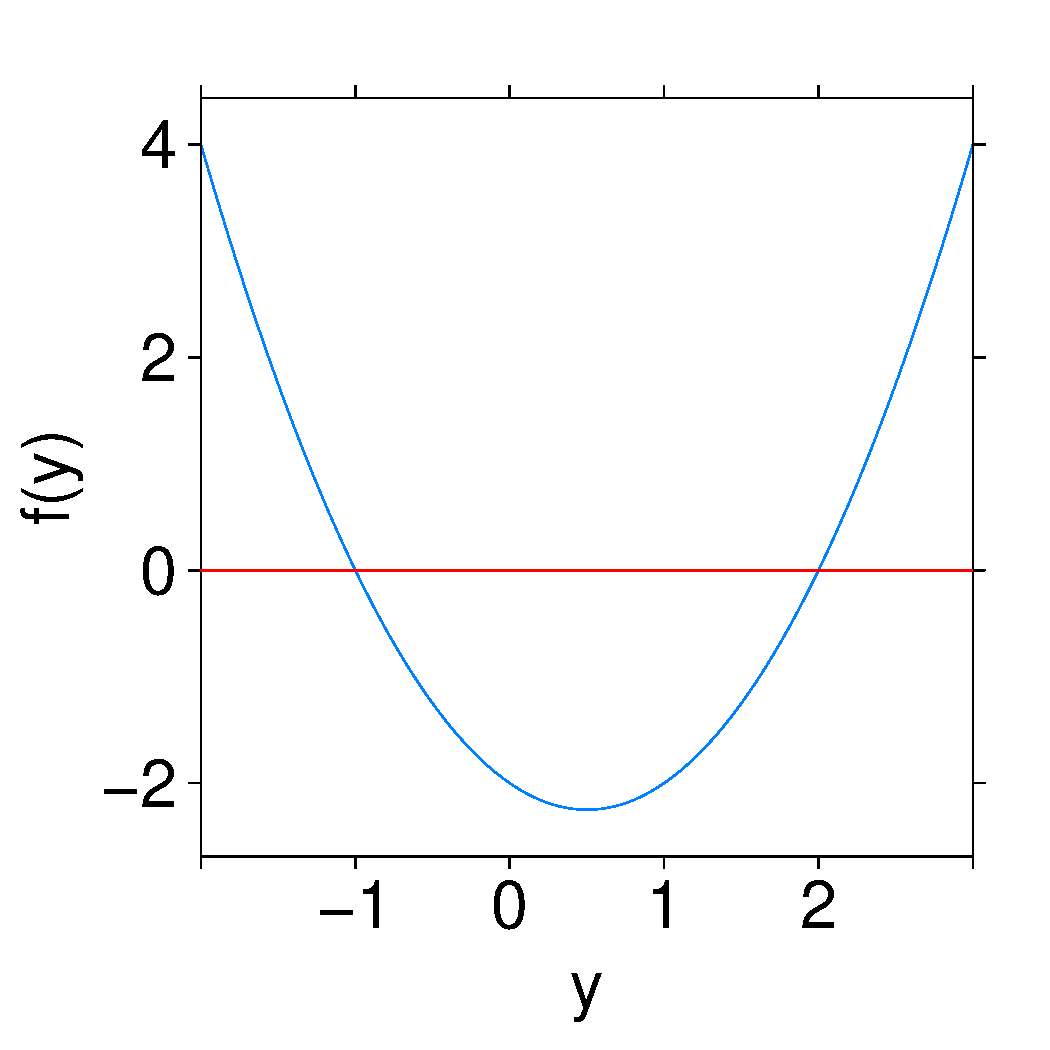
\includegraphics[width=\linewidth, keepaspectratio=true]{figure/phase.pdf}
\end{minipage}

\hspace{1cm}

\begin{minipage}[t]{0.3\textwidth}
    \begin{itemize}
        \item What is the relationship of the equilibria of $y' = 
        y^2 - y - 2$ to this curve?
    \end{itemize}
\end{minipage}

\end{frame}

\end{document}
